\documentclass{report}


%%%%%%%%%%%%%%%%%%
%   Liste des packages utilisés  %
%%%%%%%%%%%%%%%%%%

% (oui y'en a 95% qui sont inutiles ^^)

\usepackage{amssymb}
\usepackage{array}
\usepackage{hyperref}
\usepackage{booktabs}
\usepackage{multirow}
\usepackage{float}
\usepackage{lmodern} %Pack de police
\usepackage{color}
\usepackage[dvipsnames]{xcolor}
\usepackage{graphicx}
\usepackage[utf8x]{inputenc}
\usepackage[T1]{fontenc}
\usepackage{natbib}
\usepackage[francais]{babel}
\usepackage{caption}
\usepackage{listings}
\usepackage{booktabs}
\usepackage[top=2cm, bottom=2cm,left=2cm, right=2cm]{geometry}
\usepackage{blindtext}
\usepackage{setspace}
\usepackage{graphicx}
\usepackage{titlesec, blindtext, color} % titres spéciaux + couleur pour les chapter
\usepackage{fancyhdr}

% on transforme les chapters en juste le numéro suivi du titre, avec un barre grisse
\definecolor{gray75}{gray}{0.75}
\newcommand{\hsp}{\hspace{20pt}}
\titleformat{\chapter}[hang]{\Huge\bfseries}{\thechapter\hsp\textcolor{gray75}{|}\hsp}{0pt}{\Huge\bfseries}


%\titleformat{\chapter}[display]
%	{\normalfont\huge\bfseries}{}{0pt}{\Huge}

\titlespacing*{\subsection}{0pt}{2.0ex plus 1ex minus .2ex}{0.5ex plus .2ex}
\titlespacing*{\subsubsection}{0pt}{1.0ex plus 1ex minus .2ex}{0.5ex plus .2ex}


\makeatletter
\newcommand\footnoteref[1]{\protected@xdef\@thefnmark{\ref{#1}}\@footnotemark}
\makeatother


%Définition du style des bords de page
\pagestyle{fancy}
\renewcommand{\chaptermark}[1]{\markboth{\bsc{\thechapter{}- } #1}{}}
\lhead{}
\chead{}
\rhead{\leftmark}
\lfoot{Groupe n\up{o}2}
\cfoot{}
\rfoot{Page \thepage}

\fancypagestyle{plain}{%
    \lhead{}
    \chead{}
    \rhead{}
    \renewcommand{\headrulewidth}{0pt}
    \lfoot{Groupe n\up{o}2}
    \cfoot{}
    \rfoot{Page \thepage}
}

\begin{document}


%%%%%%%%%%%
%  Page de garde  %
%%%%%%%%%%%
\begin{titlepage}


		\begin{spacing}{1.5}
			\begin{minipage}{0.4\textwidth}
					
\includegraphics[width=3cm]{logo.png}
			\end{minipage}
			\begin{minipage}{0.5\textwidth}\raggedleft
					Projet Picross\\
			\end{minipage}
						\vspace*{\fill}

		\end{spacing}
	

	
	\begin{center}
		\begin{spacing}{2}
		    \hrule \vspace{1cm}
			\textbf{\Huge Application de création et d'aide à la résolution de puzzle \textit{picross}}\\[0.5cm]
			\textbf{\huge Dossier d'analyse et de conception} \\
			\vspace{1cm}
			\hrule

			\vspace*{\fill}
		\end{spacing}

		\begin{spacing}{1.15}
			\large\textbf{Groupe n\up{o}2} :\\
			\large
			\textsc{Brinon} Baptiste\\
			\textsc{Brocherieux} Thibault\\
			\textsc{Cohen} Mehdi\\
			\textsc{Debonne} Valentin\\
			\textsc{Lardy} Anthony\\
			\textsc{Mottier} Emeric\\
			\textsc{Pastouret} Gilles\\
			\textsc{Pelloin} Valentin\\
			\vspace*{\fill}
			%\textbf{Groupe n\up{o}2} \\
			\textnormal{\large Licence Informatique\\ Le Mans Université\\ \today}
		\end{spacing}
		
	\end{center}
\end{titlepage}


%%%%%%%%%%
%    Sommaire    %
%%%%%%%%%%
\renewcommand{\contentsname}{Sommaire}
\tableofcontents
\thispagestyle{empty}
\thispagestyle{plain}

\chapter{Présentation}
\thispagestyle{empty}
\thispagestyle{plain}

	\section{Introduction}

		Dans le cadre de l'unité d'enseignement "Génie logiciel 2" de la Licence d'informatique de Le Mans Université, les étudiants de troisième année sont amenés à travailler sur un projet de développement d'une application.
		
		Ce document permet de présenter les solutions au cahier des charges, ainsi que l'architecture du programme demandé. Celui-ci est divisé en plusieurs parties : l’architecture du jeu, la gestion d'une partie, l'aide à la résolution du picross, %la gestion des statistiques du joueur (scores, niveaux débloqués, …)% ainsi que l’interface graphique. Ce document décrit aussi l'utilisation du temps qui nous est imparti. 

	
 	\section{Objectif de l'application}		
		Nous devons réaliser un jeu de type picross (aussi appelé \textit{nonogramme}, \textit{logigramme} ou \textit{hanjie}) permettant à un utilisateur de résoudre des grilles et de l'aider dans sa réalisation.
		
	\section{Outils}
		
		Afin de réaliser notre application de \textit{picross}, nous utilisons plusieurs outils.
		
	LaTeX est utilisé pour rédiger et mettre en forme les différents livrables avant de les convertir en format PDF. 
	
    \textit{Git} et \textit{GitHub} permettent le partage d'informations et la mise en commun du code ainsi que les livrables associés. Nous nous servons de \textit{Discord} afin de communiquer au sein du groupe, partager nos idées, nos informations et notre travail.

	Pour concevoir les différents diagrammes UML, nous avons recours au logiciel \textit{Astah} et au site internet \textit{Tom's Planner}\footnote{Site web de \textit{Tom's Planner} : \url{http://tomsplanner.fr/}}.

	Afin de créer les maquettes du logiciel (disponibles en Annexe) permettant d’avoir un rendu de la future interface graphique, nous avons utilisé le logiciel \textit{Balsamiq}\footnote{Nos maquettes sont disponibles ici : \url{https://balsamiq.cloud/sxl7v/pw3tb/r599E}}.

	Pour simplifier la vérification de la qualité du code produit, nous utilisons Code Climate (maintenabilité) ainsi que Travis CI (compilation et tests).

	Le langage de programmation Ruby est utilisé pour programmer le logiciel, incluant une documentation générée par \textit{RDoc}\footnote{\label{rdoc}Notre documentation en temps réel est disponible à l'adresse \url{https://picross.vlntn.pw/doc/}}. L’utilisation des bibliothèques de \textit{GTK} sera utilisé pour la réalisation des interfaces graphiques.
	
	\subsection{Gems utilisés}
	Nous utilisons les \textit{gems} Ruby suivants:
	\begin{description}
	\item[RSpec :] écriture et compilation des tests unitaires
	\item[simplecov :] calcul et affichage du taux de couverte des tests unitaires
	\item[RDoc :] génération de la documentation en ligne \footnoteref{rdoc}
	\item[hanna-bootstrap :] thème responsive pour \textit{RDoc}
	\item[rake :] gestions des taches automatiques de notre projet (compilation de la documentation, tests unitaires)
	\item[rmagick :] conversion automatique d'images de picross trouvés sur internet
	\item[gtk3] : liens Ruby vers les bibliothèques d'interface graphique GTK3
	\item[Bundler :] installation automatique de tous les \textit{gems}
	\end{description}

		
\chapter{Conception générale}
\thispagestyle{empty}
\thispagestyle{plain}

    \section{Diagramme de Gantt détaillé}
    
    \begin{figure}[H]
	\caption{Diagramme de \textit{Gant détaillé}}
	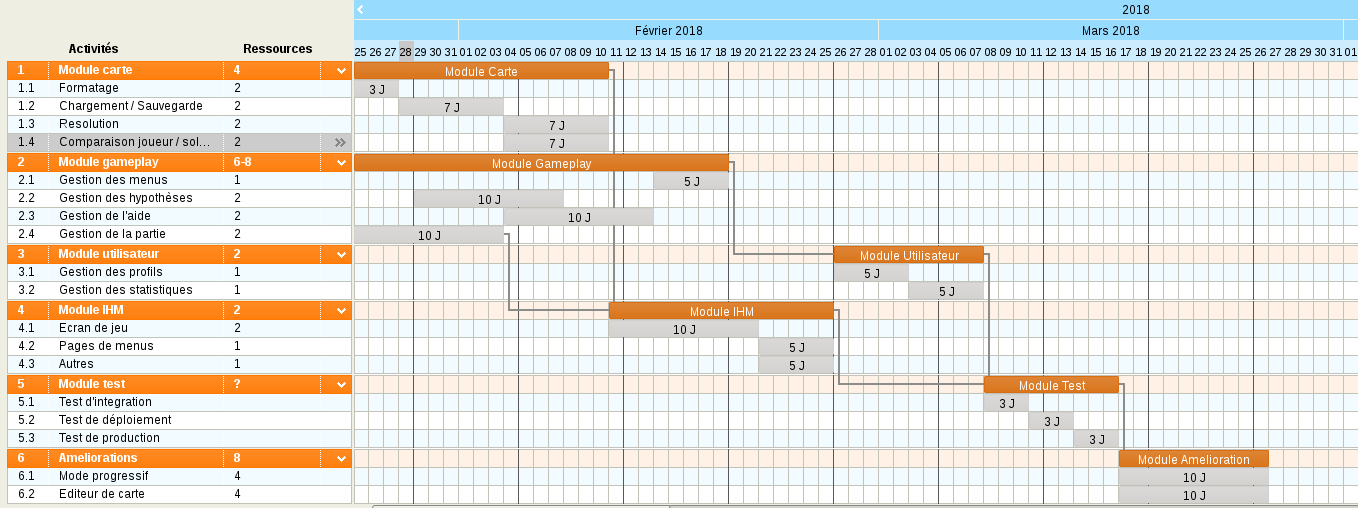
\includegraphics[width=17cm]{ganttDetaille.png}
    \end{figure}
   
     À travers ce diagramme de Gantt, nous observons l'organisation du projet sur les trois mois à venir. Le projet se découpe en plusieurs modules : carte, gameplay, utilisateur, IHM, test et améliorations.
    
    Chaque module a une durée de vie, nous lui accordons un temps de travail et un certain nombre de personnes, les modules sont également divisés en différentes étapes ce qui correspond aux fonctionnalités de l'application. 
    
    Les modules sont imbriqués les uns dans les autres, c'est-à-dire que certains dépendent d'autres modules. Sans les modules gameplay et carte réalisés, le module IHM ne peut être réalisé. 
\newpage
   \section{Besoins fonctionnels}
   
    En plus de la génération et de la gestion d'une partie, le programme doit contenir les fonctionnalités suivantes:

\begin{table}[H]
\centering
\caption{Besoins fonctionnels}
\label{table_besoins_fonctionnels}
\begin{tabular}{@{}cl@{}}
\toprule
\textbf{Catégorie}                                          & \multicolumn{1}{c}{\textbf{Besoins Fonctionnels}}                                             \\ \midrule
\multicolumn{1}{|c|}{\multirow{3}{*}{\textbf{Aide}}}        & \multicolumn{1}{l|}{BF1.1: Gagner une utilisation d'aide}                                     \\ \cmidrule(l){2-2} 
\multicolumn{1}{|c|}{}                                      & \multicolumn{1}{l|}{BF1.2 : Acheter une aide}                                       \\ \cmidrule(l){2-2} 
\multicolumn{1}{|c|}{}                                      & \multicolumn{1}{l|}{BF1.3 :  Utiliser une aide gratuite}                                                \\ \midrule
\multicolumn{1}{|c|}{\multirow{3}{*}{\textbf{Chronomètre}}} & \multicolumn{1}{l|}{BF2.1 :  Accéder au score à la fin d'une partie}                          \\ \cmidrule(l){2-2} 
\multicolumn{1}{|c|}{}                                      & \multicolumn{1}{l|}{BF2.2 : Mettre la partie en pause}                                        \\ \cmidrule(l){2-2} 
\multicolumn{1}{|c|}{}                                      & \multicolumn{1}{l|}{BF2.3: Reprendre une partie mise en pause}                                \\ \midrule
\multicolumn{1}{|c|}{\multirow{3}{*}{\textbf{Hypothèses}}}  & \multicolumn{1}{l|}{BF3.1 : Créer une hypothèse}                                              \\ \cmidrule(l){2-2} 
\multicolumn{1}{|c|}{}                                      & \multicolumn{1}{l|}{BF3.2 : Valider une hypothèse}                                            \\ \cmidrule(l){2-2} 
\multicolumn{1}{|c|}{}                                      & \multicolumn{1}{l|}{BF3.3 : Annuler une hypothèse}                                            \\ \midrule
\multicolumn{1}{|c|}{\multirow{3}{*}{\textbf{Sauvegarde}}}  & \multicolumn{1}{l|}{BF4.1 : Effectuer les sauvegardes automatiquement}                        \\ \cmidrule(l){2-2} 
\multicolumn{1}{|c|}{}                                      & \multicolumn{1}{l|}{BF4.2 : Charger automatiquement une partie à son lancement}               \\ \cmidrule(l){2-2} 
\multicolumn{1}{|c|}{}                                      & \multicolumn{1}{l|}{BF4.3 : Stocker localement les sauvegardes}                               \\ \midrule
\multicolumn{1}{|c|}{\multirow{4}{*}{\textbf{IHM}}}         & \multicolumn{1}{l|}{BF5.1 : Afficher la grille en noir et blanc}                              \\ \cmidrule(l){2-2} 
\multicolumn{1}{|c|}{}                                      & \multicolumn{1}{l|}{BF5.2 : Être compatible avec plusieurs périphériques (clavier, souris)}   \\ \cmidrule(l){2-2} 
\multicolumn{1}{|c|}{}                                      & \multicolumn{1}{l|}{BF5.3 : Mettre en valeur des indices associés aux cases remplies}        \\ \cmidrule(l){2-2} 
\multicolumn{1}{|c|}{}                                      & \multicolumn{1}{l|}{BF5.4 : Afficher la quantité de cases sélectionnées (sélection multiple)} \\ \bottomrule
\end{tabular}
\end{table}    
    
\renewcommand\thesubsection{\arabic{subsection}}
 \setcounter{secnumdepth}{5}
 
 	\subsection{Aide}
 	    \subsubsection{Gagner une utilisation d'aide}
 	            L'utilisateur a la possibilité de gagner des aides gratuites en complétant des grilles et en terminant les niveaux.
 		\subsubsection{Acheter une aide}
 			    Durant une partie, si il en a besoin, le joueur peut utiliser une aide en échange d'une pénalité de temps, sauf s'il en dispose d'une gratuite.
		\subsubsection{Utiliser une aide gratuite}
				L'utilisateur pour utiliser l'aide à tout moment en échange d'une perte de temps, sauf si celui-ci dispose d'une aide gratuite, en quel cas, l'aide n'entraînera aucune pénalité de temps.

    \subsection{Chronomètre}
			\subsubsection{Accéder au score à la fin d'une partie}
				A la fin de la partie, un nombre d'étoiles est attribué au joueur en fonction du temps écoulé.
			\subsubsection{Mettre la partie en pause}
				A n'importe quel moment de la partie, le joueur peut la mettre en pause. Elle est alors masquée.
	        \subsubsection{Reprendre une partie mise en pause}
    			Suite à une mise en pause, le joueur peut dés qu'il est prêt, relancer la partie.
	\subsection{Hypothèses}
		\subsubsection{Créer une hypothèse}
			Durant la partie, le joueur peut créer une nouvelle hypothèse en cliquant sur le bouton associé. Les cases colorées seront alors d'une couleur différente.
		\subsubsection{Valider une hypothèse}
			Lorsque l'hypothèse s'avère juste, l'utilisateur peut choisir de la valider. Les cases colorées deviennent alors noires et l'hypothèse disparaît de celles en cours.
		\subsubsection{Annuler une hypothèse}
			Lorsque l'hypothèse est fausse, l'utilisateur pour l'annuler. Les cases colorées suite à la création de l'hypothèse sont alors blanchies.
		
	\subsection{Sauvegarde}
		\subsubsection{Effectuer les sauvegardes automatiquement}
			A chaque modification de la grille, une nouvelle sauvegarde est effectuée automatiquement, sauvegardant aussi la valeur du chronomètre.
		\subsubsection{Charger automatiquement une partie à son lancement}
			Lorsque le joueur relance une partie qu'il n'avait pas terminée, le chronomètre reprends là ou il était arrêté, et la grille est affichée là ou l'avait laissée le joueur.
		\subsubsection{Stocker localement les sauvegardes}
			Les sauvegardes sont conservées sur la machine de l'utilisateur. Elles ne sont donc pas en ligne.
			
	\subsection{Interface Homme Machine}
		\subsubsection{Afficher la grille en noir et blanc}
			Les cases sont blanches, et sont colorées en noir lors de leur validation par le joueur.
		\subsubsection{Être compatible avec plusieurs périphériques}
			Le joueur peut jouer avec les périphériques qu'il désire, que ce soit seulement au clavier, seulement à la souris, ou les deux en même temps.
		\subsubsection{Mettre en valeur des indices associés aux cases remplies}
			Quand le joueur colorie des cases, le programme identifie de quel bloc de cases il s'agit et met en valeur l'indice associé, de façon à faciliter la lisibilité de la grille.
		\subsubsection{Afficher la quantité de cases sélectionnées}
			Quand l'utilisateur sélectionne plusieurs cases en une fois, un petit chiffre à coté de la souris (ou de la case sur laquelle se trouve le curseur s'il joue au clavier) indique le nombre de cases actuellement sélectionnées.
		
   \section{Diagramme de cas d'utilisations}
      
    \begin{figure}[H]
	\caption{Diagramme de \textit{Cas d’utilisation}}
	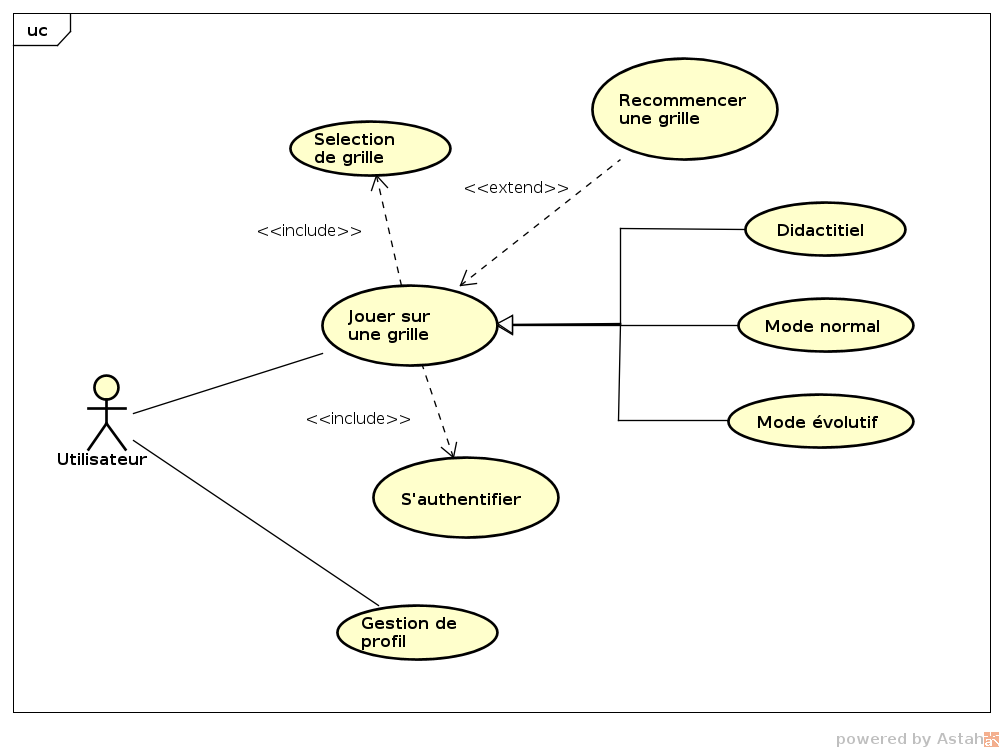
\includegraphics[width=17cm]{../UML/UseCase_diagram/UseCase1.png}
    \end{figure}
    
      %Description des cas d'utilisation

%% Reformuler
	Le but de l'utilisateur est de jouer sur une grille de \textit{picross}.
Pour cela, il doit avoir un profil. Il peut donc en créer un nouveau s'il en a envie, ou s'authentifier à un profil déjà existant.
	Le joueur doit ensuite sélectionner une grille à l'aide du menu. Il a le choix entre trois types de jeu :
	\begin{itemize}
	\item Le didacticiel, permettant d'apprendre les règles du jeu. 
	\item Le mode classique, permettant de jouer sur plusieurs grilles de tailles et difficultés variables.
	\item Le mode évolutif, agrandissant la taille de la grille au fur et à mesure que le joueur résoudra celle-ci.
	\end{itemize}
	
	À tout moment, celui-ci peut utiliser l'aide intégrée au jeu pour se débloquer. Il peut aussi choisir de recommencer la grille s'il le souhaite.

      
	\section{Mode classique}
		Dans le mode classique, le joueur a accès à plusieurs fonctionnalités. Il doit tout d'abord choisir un chapitre débloqué puis une grille. Ensuite, quand il se trouve en partie, il peut tout d'abord interagir avec la grille en cochant une case afin de se repérer dans les cases qui ne doivent pas être coloriées ou en coloriant une case. Il peut également enlever une coche ou une couleur d'une case s'il s'aperçoit qu'il s'est trompé. Il peut aussi sélectionner un groupe de cases à colorier, cocher ou vider. 
		
		Au niveau de l'interface, l'utilisateur peut, à l'aide de boutons, réinitialiser la grille s'il souhaite repartir de zéro ou la valider s'il pense l'avoir finie. S'il la réussit, il sera renvoyé dans le chapitre en cours. Il peut également utiliser différentes aides (en cliquant sur un bouton) qui diffèrent par la clarté de l'indice, leur coût et leur pénalité. Enfin, l'utilisateur peut quitter la partie quand il le souhaite, la grille est sauvegardée automatiquement.
	
	\section{Mode évolutif}
	
	Lors d'une partie en mode évolutif, le joueur choisit une des grilles du mode. Chaque grille choisie a une taille fixe de 5x5 (cases). Pour résoudre cette grille, il a accès aux mêmes fonctionnalités qu'une partie classique soit interagir avec la grille et avec l'interface.
	
    Une fois la grille réussie, celle-ci évolue en une grille plus grande (10x10) tout en gardant le coin supérieur gauche identique à la grille 5x5 réalisée par l'utilisateur (voir exemple en Annexe). Après cela, le joueur doit remplir la grille 10x10 en ayant les mêmes fonctionnalités que précédemment puis la grille évolue une nouvelle fois en 15x15 et ainsi de suite jusqu'à atteindre la taille maximale de 25x25. Une fois la grille 25x25 réussie, le joueur gagne la partie et est renvoyé sur le choix de la grille.
	
	% schéma exemple partie évolutive
	
	\section{Didacticiel}
	
	Une partie en mode didacticiel est une partie guidée afin que l'utilisateur comprenne la logique de résolution d'une partie de \textit{picross}. Les mouvements de celui-ci sont donc restreint aux coups (cocher ou colorier) que lui dit de jouer l'application.
	

	\section{Erreurs}
	
		E1: Sélection d'un chapitre non-déverrouillé
			Peut arriver lors de la sélection d'un chapitre
			Traitement: accès bloqué au chapitre et message rappelant le nombre d'étoiles manquante pour y accéder.
			
		E2: Arrêt de la partie en cours
			Peut arriver en cours de partie
			Traitement: lors du redémarrage de la partie, reprise au dernier point de sauvegarde.
		
        E3 : Lancement d'une deuxième instance
                        Dans ce cas, un message d'erreur affiche que le lancement à été bloqué.

        E4 : Quitter le menu Options sans validation de celles-ci
                         Affichage d'un message prévenant que les modifications n'ont pas été enregistrées avant de   fermer le menu. Le message propose d'enregistrer les modifications ou de les perdre, avant de quitter le menu.
	
			
  \section{Aides}

  L'utilisateur possède un nombre d'aides gratuites quand il commence à jouer et peut en récupérer en terminant un certain nombre de grille. Quand il est en jeu, il peut les utiliser afin de se débloquer sans pénalité de temps. S'il ne possède plus d'aides gratuites, alors il peut continuer d'utiliser l'aide, mais celle-ci aura un coût (en temps) proportionnel à la difficulté du picross qui sera appliqué à chaque utilisation. La difficulté influence aussi le type d'aide appliqué:
    \begin{itemize}
    \item En mode facile : coloriage de toute une ligne ou colonne
    \item En mode normal : coloriage d'une case correcte 
    \item En mode difficile : indication d'une ligne ou colonne où se trouve une case correcte non coloriée
    \end{itemize}
  
			
\chapter{Conception détaillé}
\thispagestyle{empty}
\thispagestyle{plain}

    \section{Diagramme de classe}
    
    \begin{figure}[H]
	\caption{Diagramme de \textit{Classes}}
	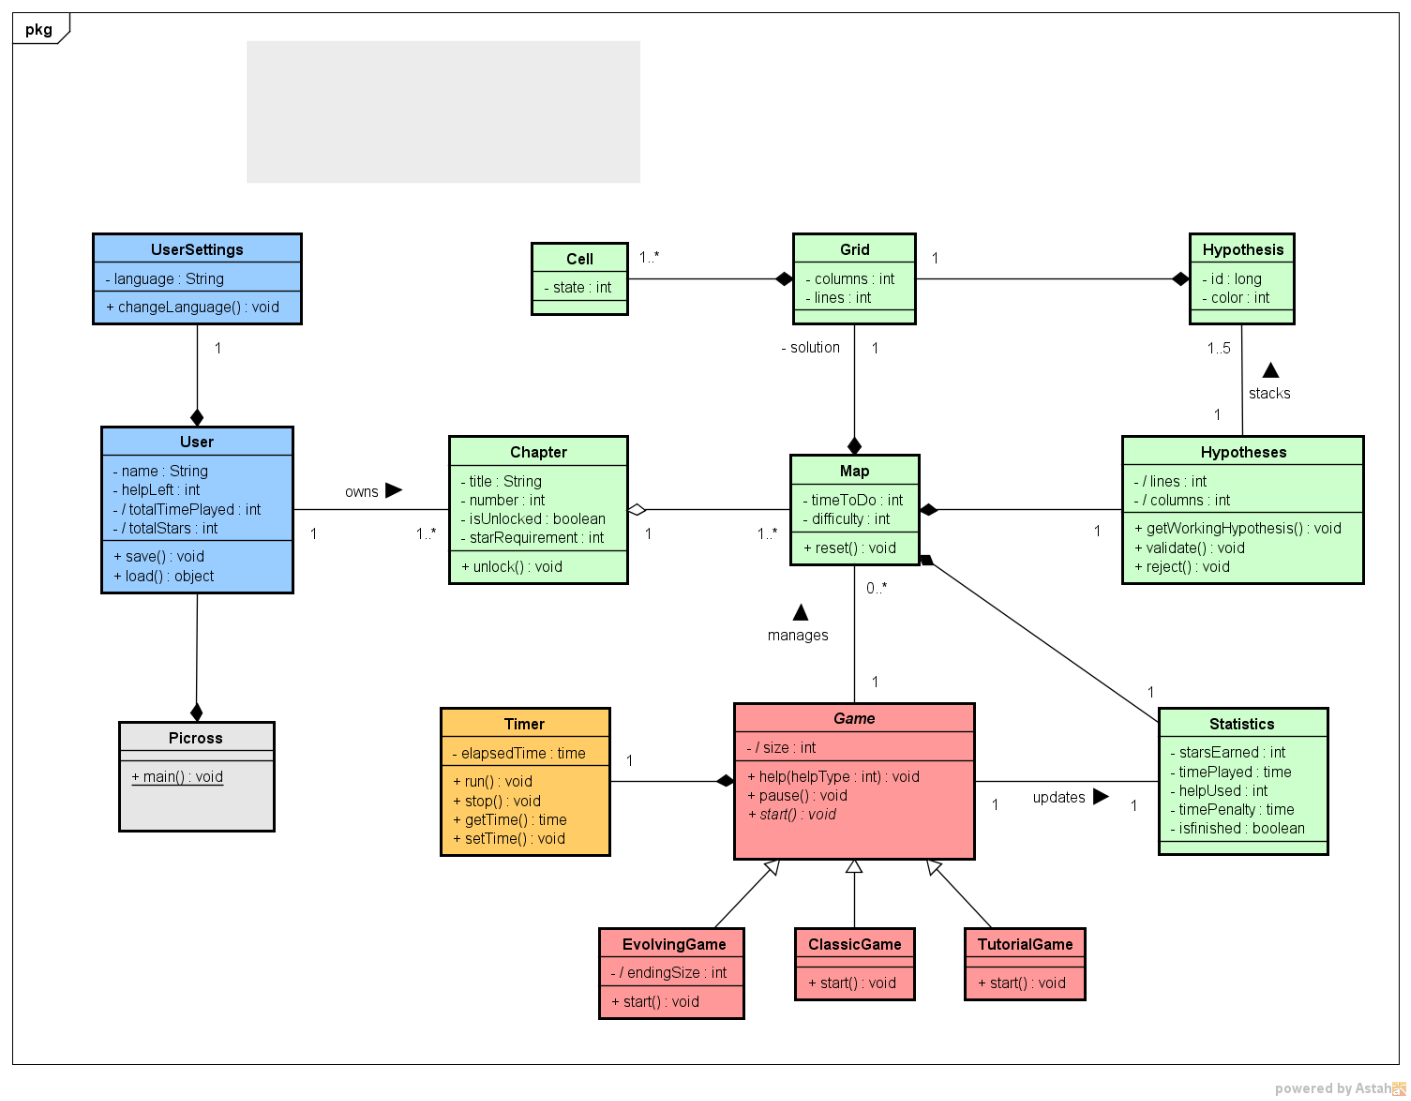
\includegraphics[width=17cm]{../UML/Class_diagram/DiagrammeClasse2b.png}
    \end{figure}
    
    	
	Le diagramme de classe ci-dessus présente les différentes classes pour notre application. Les classes nécessaires à l’interface graphique ne sont pas présentes afin de ne pas compliquer le diagramme.
	\vspace{12pt}	
	Nous avons tout d’abord la classe \textit{Picross} qui est la racine représentant l’ensemble du jeu et permettant de le lancer. Cette classe est liée à la classe \textit{User} possédant un nom, un nombre d’aides gratuites restantes ainsi que des statistiques sur le temps total joué et le nombre d’étoiles totales acquises afin de permettre l’utilisation du jeu par plusieurs personnes différentes et ainsi  avoir des sauvegardes différentes. Ces sauvegardes sont automatiques (méthode save()) et sont rechargées à la reconnexion du joueur (méthode load()). Chaque utilisateur possède des paramètres tel que celui de la langue grâce à la classe \textit{UserSettings} qu’il peut modifier par l’intermédiaire de la méthode  changeLanguage().\\
	\vspace{12pt}
	Un utilisateur possède plusieurs chapitres grâce à la classe \textit{Chapter} possédant un nom et un numéro de chapitre, une variable qui indique s’il est débloqué ou non ainsi que le nombre d’étoiles nécessaires au déverrouillage. Quand ce nombre est atteint, la méthode unlock() permet de rendre disponible ce chapitre.
	\vspace{12pt}
	Un chapitre possède plusieurs cartes de classe \textit{Map} possédant une difficulté et le temps moyen pour réaliser la grille, nécessaire au calcul du score une fois la map finie. Une map peut également être réinitialisée par l’utilisateur avec la méthode reset() afin de recommencer sa partie.\\
	\vspace{12pt}
	Une map est composée d’une grille de picross avec sa solution (classe \textit{Grid}) elle-même composée de plusieurs lignes et colonnes de cellules (classe \textit{Cell}) noires ou blanches. Chaque map possède ses propres statistiques (classe \textit{Statistiques})  composées (si la grille à été finie au moins une fois) du nombre d’étoiles gagnées, du temps joué, des aides utilisées et du temps de pénalité.\\
	\vspace{12pt}
	Une map est également composée du mode hypothèse (classe \textit{Hypotheses}) comportant plusieurs grilles d’hypothèse (classe \textit{Hypothesis}) possédant chacune un numéro et une couleur unique. Le joueur joue sur la première grille d’hypothèse et peut, s’il le souhaite, en ouvrir d’autres. Le mode hypothèse contient plusieurs méthodes : reject() permettant de rejeter l’hypothèse et donc de l’effacer, validate() permettant de valider l’hypothèse, soit de sortir de cette hypothèse tout en modifiant la grille de base avec les changements effectués dans l’hypothèse, et getWorkingHypothesis() qui permet de lancer une nouvelle hypothèse.\\
	\vspace{12pt}
	Chaque map sera gérée par une classe \textit{Game} qui gère le lancement de la partie (méthode start()) et  permet à l’utilisateur de demander une aide (méthode help()) et  mettre en pause le jeu (méthode pause()). Chaque partie possède un \textit{Timer} permettant de connaître le temps écoulé en partie ainsi que calculer le score final une fois la grille réussie. Il existe trois catégories de Game : une pour le mode de jeu tutoriel, une pour le mode classique et une pour le mode évolutif.

\chapter{Annexes}
\thispagestyle{empty}
\thispagestyle{plain}

		\section{Exemple partie évolutive}
	
		Ci-joint sont présent des exemples de grilles évolutives, c'est-à-dire de grilles qui s'agrandissent au fil de la partie.
		Deux exemples de grilles sont disponibles sous forme de gif animé aux liens suivants :
		 \begin{itemize}
    		 \item \url{https://picross.vlntn.pw/Documents/Images/cat.gif}
   	   	 \item \url{https://picross.vlntn.pw/Documents/Images/mouse.gif}
		 \end{itemize}
		
		Le premier gif est également disponible sous format d'un ensemble d'images :
	
		\begin{figure}[H]
	       	 	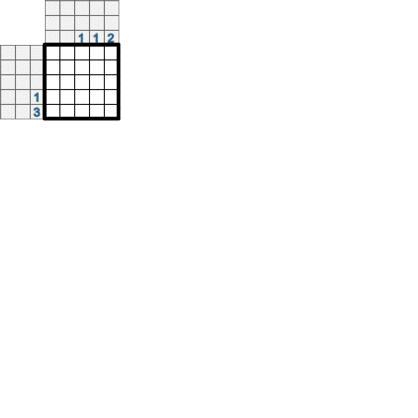
\includegraphics[width=5cm]{../Images/cat/cat1.png}
			\hspace{1cm}
          		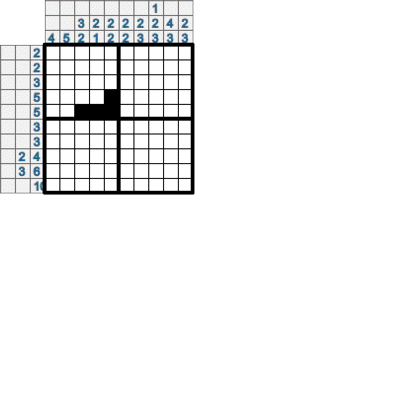
\includegraphics[width=5cm]{../Images/cat/cat2.png}
			\hspace{1cm}
			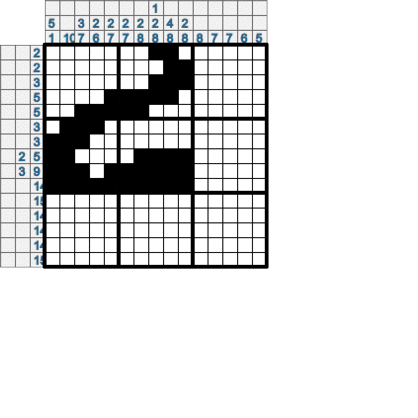
\includegraphics[width=5cm]{../Images/cat/cat3.png}
			\hspace{1cm}
          		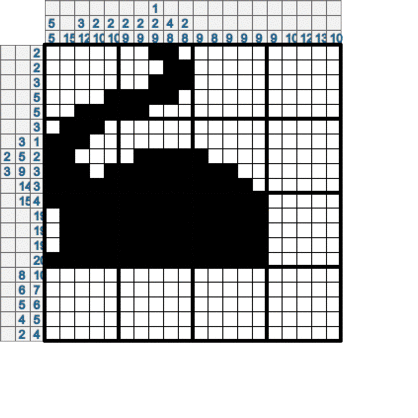
\includegraphics[width=5cm]{../Images/cat/cat4.png}
			\hspace{1cm}
          		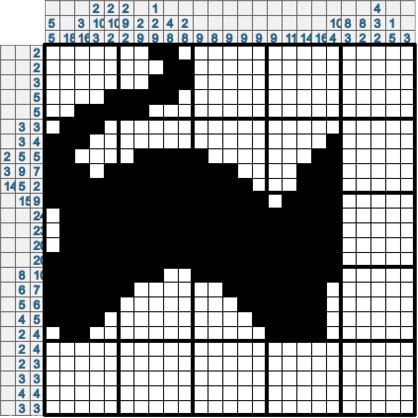
\includegraphics[width=5cm]{../Images/cat/cat5.png}
			\hspace{1cm}
			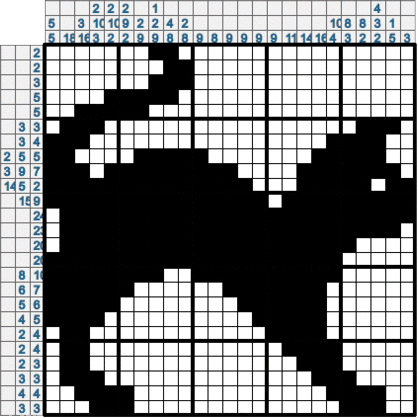
\includegraphics[width=5cm]{../Images/cat/cat6.png}
		\end{figure}
		
	
	\section{Maquettes de l'interface}
      
      		Ci-dessous les maquettes réalisées pour l'interface de notre application en français. 
      		
      		Lorsque le joueur lance l'application, il tombe sur l'écran (1) lui demandant de rentrer son pseudo pour permettre à chaque joueur d'avoir son propre profil. S'il rentre un pseudo déjà existant, il charge son profil avec ses statistiques et ses chapitres débloqués sinon un nouveau profil est créer. 
      		
      		L'utilisateur arrive ensuite sur la page d'accueil du logiciel (2) lui permettant de choisir parmi les différentes fonctionnalités. Le bouton \textit{Quitter} ferme l'application. 
      		
      		Le bouton \textit{Options} renvoit sur la page d'options (3) qui permet à l'utilisateur de modifier ses préférences de jeu. 
      		
      		Le bouton \textit{Règles}  permet d'afficher les règles générales du \textit{picross} (4). L'utilisateur peut voir ses statistiques et celles des autres utilisateurs en cliquant sur le bouton \textit{Classement}. 
      		
      		Enfin, en cliquant sur le bouton \textit{Jouer}, l'utilisateur est envoyé sur la sélection du  chapitre (5) comportant tout les chapitres du jeu, didacticiel et mode évolutif inclus. 
      		
      		Après avoir choisi un chapitre, il arrive sur la sélection de la grille (6) ainsi que le nombre d'étoiles obtenues sur les grilles déjà réussies. Lorsqu'il a choisi sa grille, la partie commence (7).
		
		
	\begin{figure}[H]
    		\begin{minipage}[c]{.46\linewidth}
       			\centering
       			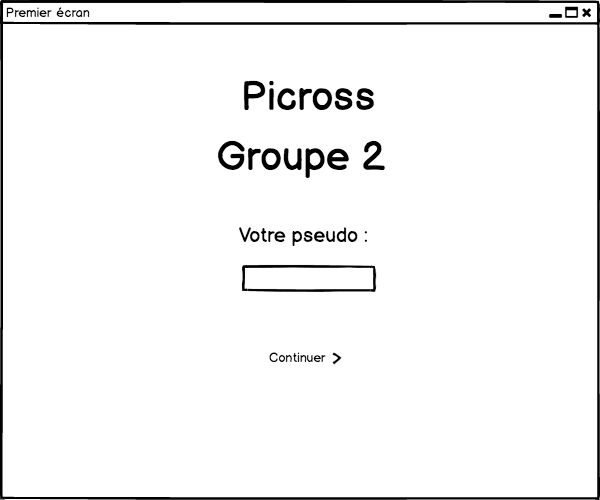
\includegraphics[width=8cm]{Maquettes/Premier_ecran.png}
        			\caption{(1) Écran de connexion}
    		\end{minipage}
    		\hfill
   		\begin{minipage}[c]{.46\linewidth}
        			\centering
       			 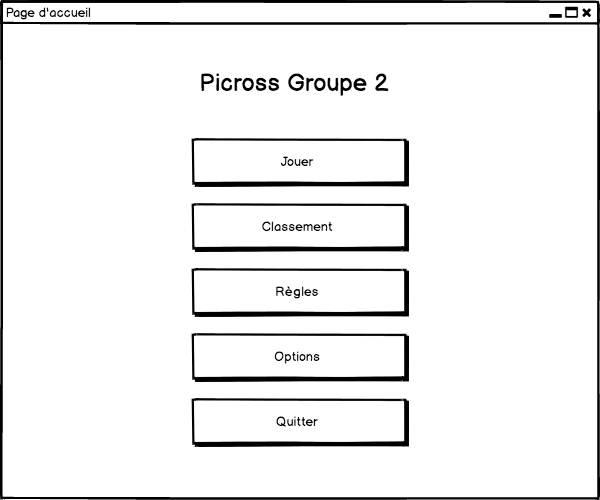
\includegraphics[width=8cm]{Maquettes/Page_Accueil.png}
        			\caption{(2) Page d'accueil}
    		\end{minipage}
	\end{figure}
	
	\begin{figure}[H]
    		\begin{minipage}[c]{.46\linewidth}
       			\centering
       			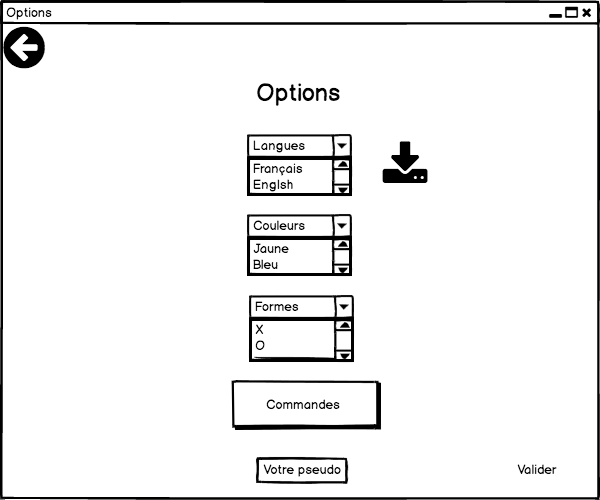
\includegraphics[width=8cm]{Maquettes/Options.png}
        			\caption{(3) Options}
    		\end{minipage}
    		\hfill
   		\begin{minipage}[c]{.46\linewidth}
        			\centering
       			 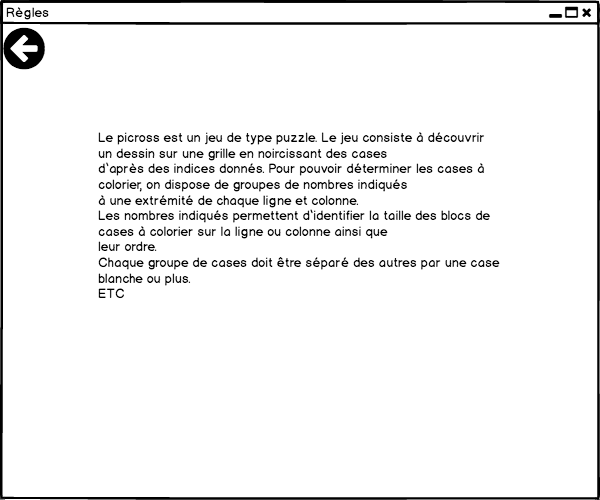
\includegraphics[width=8cm]{Maquettes/Regles.png}
        			\caption{(4) Règles}
    		\end{minipage}
	\end{figure}
	
	\begin{figure}[H]
    		\begin{minipage}[c]{.46\linewidth}
       			\centering
       			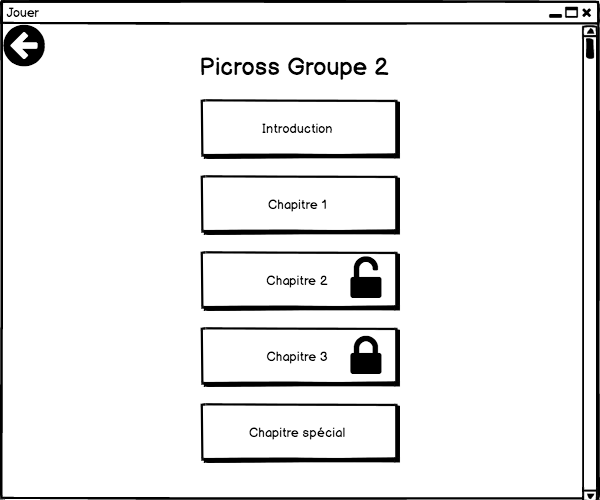
\includegraphics[width=8cm]{Maquettes/Jouer.png}
        			\caption{(5) Sélection du chapitre}
    		\end{minipage}
    		\hfill
   		\begin{minipage}[c]{.46\linewidth}
        			\centering
       			 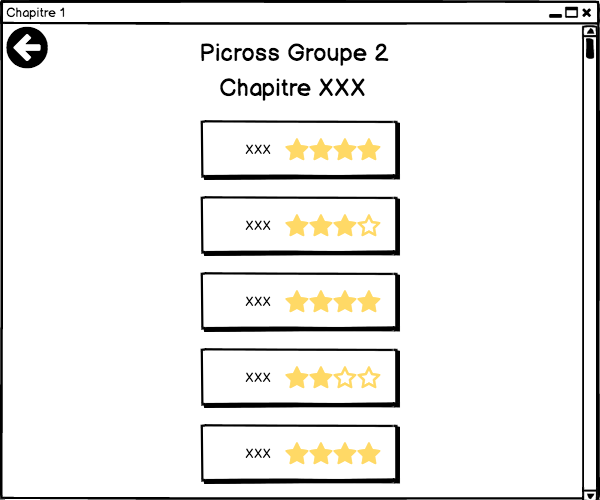
\includegraphics[width=8cm]{Maquettes/Chapitre_1.png}
        			\caption{Sélection de la grille}
    		\end{minipage}
	\end{figure}
	
	 \begin{figure}[H]
	 	\centering
		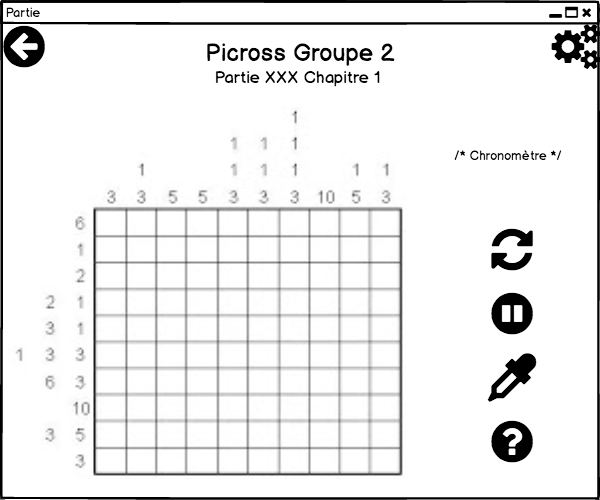
\includegraphics[width=8cm]{Maquettes/Partie.png}
		\caption{Partie}
    	\end{figure}


\end{document}
